\chapter{Search for heavy scalars and pseudoscalars in \ttbar}
\label{ch:ah}

\section{Introduction}
\label{sec:ah:intro}

As explained in \cref{sec:theory:hext}, additional spin-0 particles are predicted in many attractive extensions of the Standard Model, and searches for such particles at the LHC have potential of discovering hints for new physics. Oftentimes, such models predict Yukawa-type couplings for the new particles to SM fermions, which scale with the fermion mass. It is thus natural to search for interactions of new spin-0 states with the heaviest fundamental particle in the SM: the top quark.

In particular, if the mass of any such new state is larger than double the top quark mass, it can decay to a \ttbar final state. This decay channel will be dominant in many scenarios. If the new state is produced in gluon fusion, the resulting process will interfere with SM \ttbar production as discussed in \cref{sec:theory:ttbar}, leading to an interference pattern in the invariant \ttbar mass that can be probed experimentally.

To do so, a generic model describing the new particles is defined, containing two new spin-0 states A and H which both couple solely to the top quark via a pseudoscalar (for A) and a scalar (for H) Yukawa interaction. The Lagrangian reads

\begin{equation}
\label{eq:ah:lagrangian}
\begin{split}
    \mathcal{L}_{\AH} =& \, \frac{1}{2} (\partial_\mu A ) (\partial^\mu A ) +\frac{\mA^2}{2} A^2  
    + i  \gAtt \, \frac{\mt}{v} \bar t  \gamma_5 \, t  \, A \\
    & + \frac{1}{2} (\partial_\mu H ) (\partial^\mu H ) +\frac{\mH^2}{2} H^2  
    -  \gHtt \, \frac{\mt}{v} \bar t \, t  \, H \,
\end{split}
\end{equation}

Here, \mA and \mH are the masses of the new particles, \gAtt and \gHtt are the coupling modifiers for the top quark Yukawa couplings, \mt is the top quark mass, and $v$ is the vacuum expectation value of the SM Higgs boson. 

This model assumes that the two states A and H do not mix, which is equivalent to the assumption that there is no CP violation [??]. Apart from this assumption, it is fully generic and can be mapped onto any of the models discussed in \cref{sec:theory:hext}, provided that only couplings to the top quark are considered. This makes it ideal for an experimental search, as results presented using this model can be easily reinterpreted in various models of interest.

In addition to the masses and coupling modifiers, the decay widths \wA and \wH of the two particles are also considered as free parameters, yielding six free parameters total. This is because, due to interactions with other SM particles besides the top quark, or with additional BSM particles, concrete models (e.g. the 2HDM) will predict different decay widths then the natural width expected in the simplified model. In particular, if either or both of the particles is to be considered a dark matter mediator, it will have a significant branching ratio to dark matter particles, increasing its absolute width.

This chapter presents a search for new spin-0 states with either scalar or pseudoscalar interactions with the top quark, using the full Run~2 dataset ($L= \SI{138}{\fbinv}$). The work done as part of this thesis focused on the dilepton decay channel of \ttbar, which is thus described in detail in~\cref{sec:ah:setup,sec:ah:reweighting,sec:ah:prefit}. It was then combined with a similar analysis of the \ljets decay channel, and the results of both the dilepton channel alone and the combination are discussed in \cref{sec:ah:etat,sec:ah:limits}.

\section{Analysis setup}
\label{sec:ah:setup}

\subsection{Datasets}

\paragraph{Experimental data.} 
The analysis is performed using the full CMS Run~2 ultra-legacy (UL) dataset, which is the final, re-reconstructed and recalibrated dataset recommended by CMS for physics analyses. It is split into the three datataking years of Run~2: 2016, 2017 and 2018, where 2016 is again split into two parts, denoted as "2016pre" and "2016post". \todo{why is 2016 split} 

A similar combination of dilepton and single-lepton triggers as in \cref{sec:ttxs:datasets} is used for all years, with the \pt thresholds varying slightly between datataking eras, as shown in \cref{tab:ah:triggers}. 

\begin{table}
\centering
\begin{tabular}{|c|c|c|}
    \hline
    Trigger & Year & Lepton \pt requirement \\
    \hline
    \multirowcell{3}{single-e} & 2016 & $e(\pt > \SI{27}{\GeV})$ \\
    & 2017 & $e(\pt > \SI{35}{\GeV})$ \\
    & 2018 & $e(\pt > \SI{32}{\GeV})$ \\
    \hline
    \multirowcell{3}{single-$\mu$} & 2016 & $\mu(\pt > \SI{24}{\GeV})$ \\
    & 2017 & $\mu(\pt > \SI{27}{\GeV})$ \\
    & 2018 & $\mu(\pt > \SI{24}{\GeV})$ \\
    \hline
    \multirowcell{2}{e$\mu$} & \multirowcell{2}{all} & $e(\pt > \SI{12}{\GeV})$ and $\mu(\pt > \SI{23}{\GeV})$ or \\
    & & $e(\pt > \SI{23}{\GeV})$ and $\mu(\pt > \SI{8}{\GeV})$ \\
    \hline
    ee & all & $e_1(\pt > \SI{23}{\GeV})$ and $e_2(\pt > \SI{12}{\GeV})$ \\
    \hline
    $\mu \mu$ & all & $\mu_1(\pt > \SI{17}{\GeV})$ and $\mu_2(\pt > \SI{8}{\GeV})$ \\
    \hline
\end{tabular}
\caption{\textbf{Trigger \pt thresholds.} Overview of the used triggers in the three datataking years, as well as their lepton \pt thresholds.}
\label{tab:ah:triggers}
\end{table}

\paragraph{Background simulation.}
Since this analysis is, in essence, a search for interference patterns of the signal with the SM \ttbar background, it is clear that a large irreducible background is expected. As a result, it is essential that the SM Monte Carlo simulation is as both theoretically precise and has sufficient statistics, and that any remaining imprecisions are covered by the systematic uncertainty model.

The SM \ttbar background is again simulated at NLO in QCD with the \texttt{hvq} process from the  MC generator package \textsc{Powheg Box v2} and interfaced to \textsc{Pythia 8} for showering. Similar settings as in \cref{sec:ttxs:datasets} have been used. To achieve the necessary precision, the NLO simulation is reweighted to higher orders in both QCD and electroweak (EW) processes, which is described in \cref{sec:ah:ttbarweights}.

In addition, several minor backgrounds are included, a summary of which can be found in \cref{tab:ah:simulation}. Of note here is the Z+jets background, which is simulated at NNLO in QCD using the MiNNLO method in \textsc{Powheg Box v2}. It was found here that the higher-order corrections are relevant to the analysis especially for low values of the invariant dilepton mass \mll.

\begin{table}
\centering
\begin{tabular}{|c|c|c|}
    \hline
     Process & QCD order & ME Generator \\
     \hline
     \ttbar & NLO & {Powheg v2} (\texttt{hvq}) \\
     tW & NLO & {Powheg v2} (\texttt{ST\_wtch}) \\
     Z+jets & NNLO & {Powheg v2} (\texttt{Zj} MiNNLO) \\
     $t$-channel single top & NLO & {Powheg v2} (\texttt{ST\_tch}) + {MadSpin} \\
     $s$-channel single top & NLO & {MG5\_aMC@NLO} \\
     $\ttbar \mathrm{W}$ & NLO & {MG5\_aMC@NLO} \\
     $\ttbar \mathrm{Z}$ & NLO & {MG5\_aMC@NLO} \\
     WW, WZ \& ZZ & LO & {Pythia 8.2} \\
     \hline
     \AH signal & LO & {MG5\_aMC@NLO} \\
     \etat signal & LO & {MG5\_aMC@NLO} \\
     \hline
\end{tabular}
\caption{\textbf{Simulated background and signal samples.} An overview of the different background and signal processes considered, as well as the theoretical order in QCD and the ME generator used to simulate them. For all samples, \textsc{Pythia 8.2} is used for showering and hadronization.}
\label{tab:ah:simulation}
\end{table}

\todo{cross sections}

\paragraph{Signal simulation.}

The signal for the general \AH model described in \cref{sec:ah:intro} is generated at LO in QCD using \textsc{MadGraph 5} with a custom Universal FeynRules Output (UFO) model. The $p p \to \AH \to \ttbar$ resonance and the \AH-SM interference are simulated separately, and both are again showered with \textsc{Pythia 8}. In order to cover the phase space of the \AH model, the signals are generated for all combinations of the following values of the \AH masses and widths:

\begin{equation}
\begin{split}
    m_{\AH} &\in \{ 365, 400, 500, 600, 800, 1000 \} \, \si{\GeV} \\
    \Gamma_{\AH} / m_{\AH} &\in \{ 2.5, (5), 10, 25 \} \, \%
\end{split}
\end{equation}

Samples with a width of $5\%$ were generated only for masses of \SI{400}{\GeV}, which leads to 38 signal points total. In addition, samples for the pseudoscalar case only were generated with

\begin{equation}
    \mA \in \{ 450, 550, 700, 900 \} \, \si{GeV}, \quad \wA / \mA = 9 \, \%.
\end{equation}

All of these samples were combined and used reweighted at matrix element level to obtain also phase space points between these mass and width values, as described further in \cref{sec:ah:mereweighting}.

In order to probe possible non-perturbative effects in \ttbar, an additional signal sample is generated using the color-singlet \etat toy model described in \citere{Fuks:2021xje}, using a UFO model provided by the authors.

For all signal and background samples, the detector response is simulated with \textsc{Geant 4} and the full CMS simulation and reconstruction chain as described in [??] is performed.

\subsection{Object definition}
\label{sec:ah:objects}

\paragraph{Leptons.} 

All electrons and muons are required to have $\pt > \SI{20}{\GeV}$ and $\abseta < 2.4$ to be considered for the analysis. Similar to \cref{sec:ttxs:objects}, electrons in the transition region between barrel and endcaps in the ECAL are removed, and additional ID critera are applied for both types of leptons.

For electrons, the multivariate classifier (MVA)-based ID described in \citere{CMS:EGM-17-001} is used at a working point giving 90 \% background rejection. This ID already includes an isolation requirement as part of the MVA training, and no further requirement is applied.

For muons, the same cut-based ID from \citere{CMS:MUO-16-001} as in \cref{sec:ttxs:objects}, also at the tight working point, is used, and the same isolation requirement using a cone size of $\Delta R < 0.4$ is applied in addition.

\paragraph{Jets.} 

Jets are again reconstructed using the anti-$k_T$ algorithm~\cite{Cacciari:2008gp} with a distance parameter of $0.4$. They are required to fulfill $\pt > \SI{20}{\GeV}$, $\abseta < 2.4$, and have a minimum distance of $\Delta R > 0.4$ from all leptons passing the above criteria in the event.

The \textsc{DeepJet} algorithm~\cite{DeepJet:2020}, same as in \cref{sec:ttxs:objects}, is used to identify jets originating from the showering and hadronization of b quarks. The medium working point of \textsc{DeepJet} in CMS, corresponding to an identification efficiency of XX \% is chosen~\cite{CMS:BTV-16-002}.

\paragraph{Missing transverse momentum.}

In the dileptonic decay of \ttbar, the two neutrinos can not be measured experimentally, and escape the detector unseen. However, their presence can be inferred from momentum conservation: In a proton-proton collision, the longitudinal component of the incoming partons in the hard scattering process is unknown, while the transverse component can be assumed to be close to zero. Thus, the missing transverse momentum \ptmissvec can be inferred as the negative vectorial sum of all reconstructed objects (jets, leptons and photons)~\cite{CMS:JME-17-001}. Along with the leptons and jets, it will be used to reconstruct the \ttbar system.

\subsection{Event selection}

Events are selected with exactly two leptons of opposite electric charge and sorted into three channels (\ee, \emu and \mumu) by lepton flavor, similar to \cref{sec:ttxs:channels}. The two leptons need to fulfill $\pt > \SI{25}{\GeV}$ and $\pt < \SI{20}{\GeV}$ for the leading and subleading lepton, respectively, and their invariant mass is required to be $\mll > \SI{20}{\GeV}$ in order to reject background from $\gamma^*$+jets production and low-mass resonances. 

In all channels, at least two jets with $\pt > \SI{30}{\GeV}$ are required, of which at least one needs to be b-tagged. Furthermore, in the same-flavor lepton channels (\ee and \mumu), additional cuts are applied to reject Z+jets background: Events with $|\mll - m_Z| < \SI{15}{\GeV}$, i.e. close to the Z boson mass peak, are discarded (again just as in \cref{sec:ttxs:channels}), and the magnitude of the missing transverse momentum is required to be $\ptmiss > \SI{40}{\GeV}$.

The effect of all selection cuts can be seen in \cref{fig:ah:cutflows}.

\begin{figure}
    \centering
    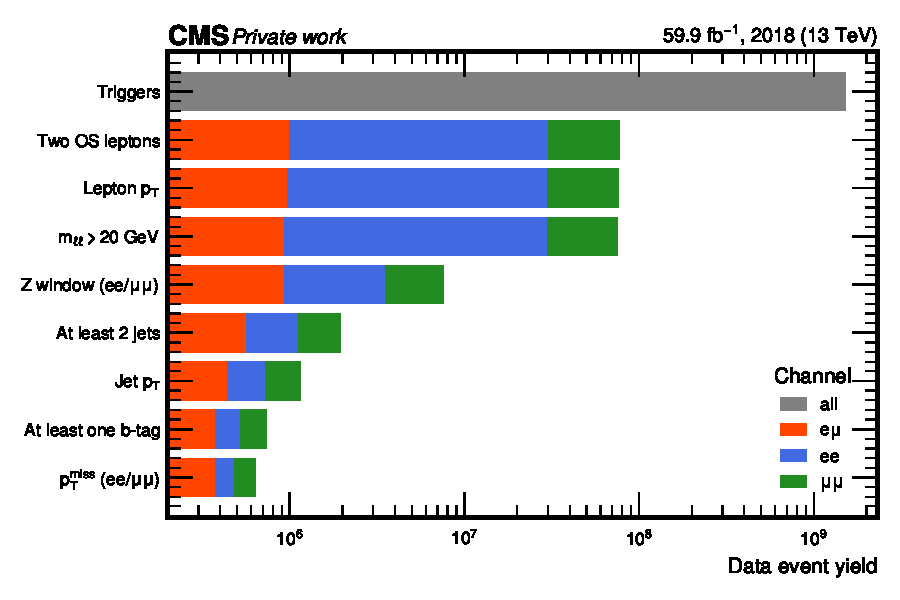
\includegraphics[width=\textwidth]{figures/ah/cutflows.pdf}
    \caption{\textbf{Selection cuts.} Shown is the data yield in 2018 (corresponding to $\Lint = \lumiVIII$) after successively applying all selection cuts. Starting with the requirement of two opposite-sign leptons, the three channels are marked with different colors.}
    \label{fig:ah:cutflows}
\end{figure}

\subsection{Experimental corrections}

Similar as in \cref{sec:ttxs:corrections}, several corrections are applied to the MC simulation in order to achieve good agreement with the data. In contrast to the \ttbar cross section measurement, where most of these corrections were derived as part of this work, many of the experimental corrections used in this chapter were provided centrally by the CMS collaboration. These will only be described very briefly; more details can be found in the associated references.

\paragraph{Trigger scale factors.}

The selection efficiency of the triggers given in \cref{tab:ah:triggers} in simulation needs to be corrected to the one measured in data. This is done via scale factors, which were centrally derived as a function of the \pt of the two leptons using the so-called cross-trigger method: Events are selected using a different set of triggers - here, a combination of jet and \ptmiss triggers - which is assumed to be fully orthogonal to the lepton triggers used for the main selection. Thus, the event sample is unbiased with respect to the lepton triggers, and the lepton trigger efficiency can be measured as the fraction of these events who pass the lepton triggers in addition to the jet/\ptmiss triggers. This is done independently for all datataking years, and the resulting difference in efficiencies is in most cases less then 1 \%.

\paragraph{Lepton scale factors.}

Differences in the efficiency for a lepton to pass the identification and isolation criteria as defined in \cref{sec:ah:objects} are measured using the tag-and-probe method, as in \cref{sec:ttxs:corrections}, and applied to simulation using scale factors binned in \pt and \abseta of the lepton. The difference in efficiency is typically on the order of 1-5 \%, with the magnitude increasing for high \abseta. For more details on this method see Refs.~\cite{CMS:EGM-17-001,CMS:MUO-16-001}.

\paragraph{Pileup reweighting.}



\paragraph{Jet energy corrections.}

\paragraph{b-tagging scale factors.}

\paragraph{ECAL pre-firing.}

\paragraph{Z+jets background normalization.}

\subsection{Reconstruction of the \ttbar system}

\subsection{Sensitive observables}

\section{Simulation reweighting}
\label{sec:ah:reweighting}

\subsection{Higher-order corrections in \ttbar}
\label{sec:ah:ttbarweights}

\subsection{Matrix element reweighting for \AH signals}
\label{sec:ah:mereweighting}

\section{Pre-fit distributions}
\label{sec:ah:prefit}

\section{Extraction of non-perturbative effects in \ttbar}
\label{sec:ah:etat}

\section{BSM limits}
\label{sec:ah:limits}

\section{Summary}

\chapter{Investigation of Axion-Like Particles decaying to \ttbar}
\label{ch:alps}

\section{Introduction and definitions}

\section{Translation of Higgs boson limits}

\section{Technical setup}

\section{Discrimination between ALPs and pseudoscalar Higgs bosons}

\section{Projected limits for ALPs}

\section{Summary}